\chapter{\ifenglish Introduction\else บทนำ\fi}

\section{วัตถุประสงค์}
\begin{enumerate}
    \item เพื่อเรียนรู้แนวคิดและหลักกาารทำงานของ DevOps ในสถาณการณ์การทำงานจริงซึ่งในองค์กรขนาดใหญ่
    \item เพื่อศึกษาเรียนรู้และปรับใช้เครื่องมือและเทคโนโลยีใหม่ ๆ ที่เกี่ยวกับ Iac (Infrastructure as Code) และ CI/CD (Continuous Integration / Continuous Deployment)
    \item เพื่อนำความรู้ที่ได้มาปรับใช้กับโปรเจคจบ ในปีการศึกษาต่อไปเพื่อเสริมการใช้ Standard ให้กับการทำงานเพื่อให้โปรเจคมีคุณภาพมากยิ่งขึ้น
    \item เพื่อฝึกกระบวณการคิดและการออกแบบระบบโครงสร้างพื้นฐานของระบบที่มีความยืดหยุ่นสูงและสามารถใช้ได้กับองค์กรทุกขนาด

\end{enumerate}

\section{\ifenglish Company History\else ประวัติความเป็นมาของบริษัท\fi}

SCB TechX \cite{techxWebsite} ก่อตั้งขึ้นจากความร่วมมือระหว่าง SCBX กลุ่มธุรกิจการเงินและเทคโนโลยีชั้นนำของไทย และ Publicis Sapient บริษัทที่ปรึกษาด้านดิจิทัลทรานส์ฟอร์เมชันระดับโลก มีจุดมุ่งหมายเพื่อมอบบริการด้านเทคโนโลยีที่ตอบสนองความต้องการของธุรกิจต่าง ๆ ตั้งแต่การสร้างนวัตกรรมและผลิตภัณฑ์ใหม่ ไปจนถึงการนำเทคโนโลยีมาเพิ่มประสิทธิภาพในการดำเนินงาน

บริษัทมีความเชี่ยวชาญในการพัฒนาโซลูชันในระดับองค์กร (Enterprise-grade solutions) ที่ปลอดภัยและรองรับการใช้งานของฐานลูกค้าจำนวนมาก นอกจากนี้ SCB TechX ยังจัดองค์กรในรูปแบบ Startup ถึงแม้จะเป็นองค์กรขนาดใหญ่ เพื่อลดความซ้ำซ้อนในการทำงานและส่งเสริมความคิดริเริ่มใหม่ ๆ ทำให้สามารถพัฒนาโซลูชันให้กับลูกค้าได้อย่างรวดเร็วและมีประสิทธิภาพ


\section{\ifenglish Company Product\else บริการและผลิตภัณฑ์ของบริษัท\fi}
SCB TechX นำเสนอนวัตกรรมที่พร้อมใช้งานหลากหลายด้าน \cite{techxProduct} ทั้งระบบยืนยันตัวตนแบบดิจิทัลด้วยระบบ KYC \cite{whatIsKYC} ซึ่งทางบริษัทจะเรียกว่า eKYC และแพลตฟอร์มทางการเงินที่หลากหลาย นวัตกรรมเหล่านี้สามารถเชื่อมต่อกับระบบของลูกค้าได้อย่างรวดเร็วและง่ายดาย พร้อมทั้งปรับแต่งตามความต้องการเฉพาะของธุรกิจ ส่งผลให้ลูกค้าของ SCB TechX สามารถเปิดตัวบริการใหม่หรือยกระดับการให้บริการได้อย่างทันท่วงที

นอกจากนี้ SCB TechX ยังให้บริการที่ครอบคลุมด้านการให้คำปรึกษาทางเทคโนโลยี (Technology Consulting), โซลูชันด้านโครงสร้างพื้นฐานและแพลตฟอร์ม (Infrastructure \& Platforms), โซลูชันคลาวด์ (Cloud Solutions), แพลตฟอร์ม DevOps as a Service ที่ครบวงจร (xPlatform), การจัดการข้อมูลและความปลอดภัย (Data \& Security), และโซลูชันด้านข้อมูลและ AI (TechX Data \& AI Solutions) ที่ออกแบบมาเพื่อรองรับและเสริมสร้างศักยภาพให้กับธุรกิจในยุคดิจิทัล

\clearpage

\section{\ifenglish Organization\else ผู้บริหารของบริษัท\fi}
\begin{table}[ht]
    \centering
    \begin{tabular}{c||c}
        \textbf{Name}          & \textbf{Position}            \\
        \hline
        \hline
        Trirat Suwanprateeb    & Chief Executive Officer      \\
        Jonathan Sharp         & Chief Technology Officer     \\
        Pavarej Hwangdee       & Chief Product Officer        \\
        Yuwanan Buranaanusorn  & Chief Finance Officer        \\
        Jaruwan Lueponglukkana & Chief Human Resource Officer \\
    \end{tabular}
    \caption{ตารางแสดงตำแหน่งผู้บริหารของบริษัท}
\end{table}
\begin{figure}[ht]
    \begin{center}
        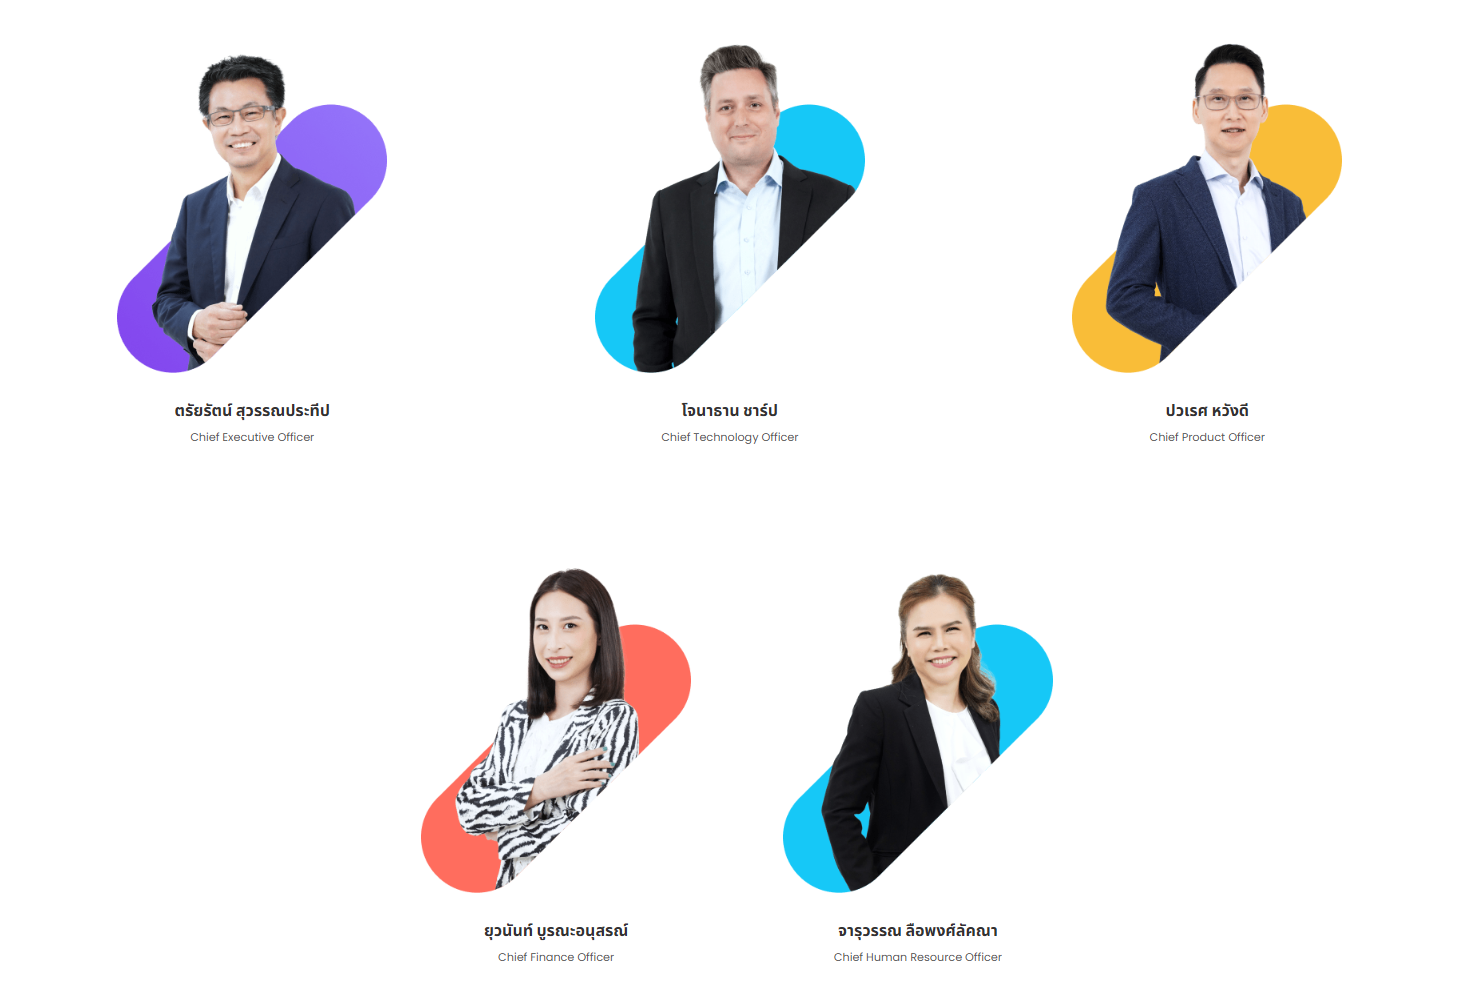
\includegraphics[scale=0.35]{images/org.png}
    \end{center}
    \caption[ผู้บริหารและตำแหน่งของบริษัท]{ผู้บริหารและตำแหน่งของบริษัท}
\end{figure}

\clearpage

\section{งบการเงินและงบกำไรขาดทุน}
\subsection{งบการเงิน}
\begin{figure}[ht]
    \begin{center}
        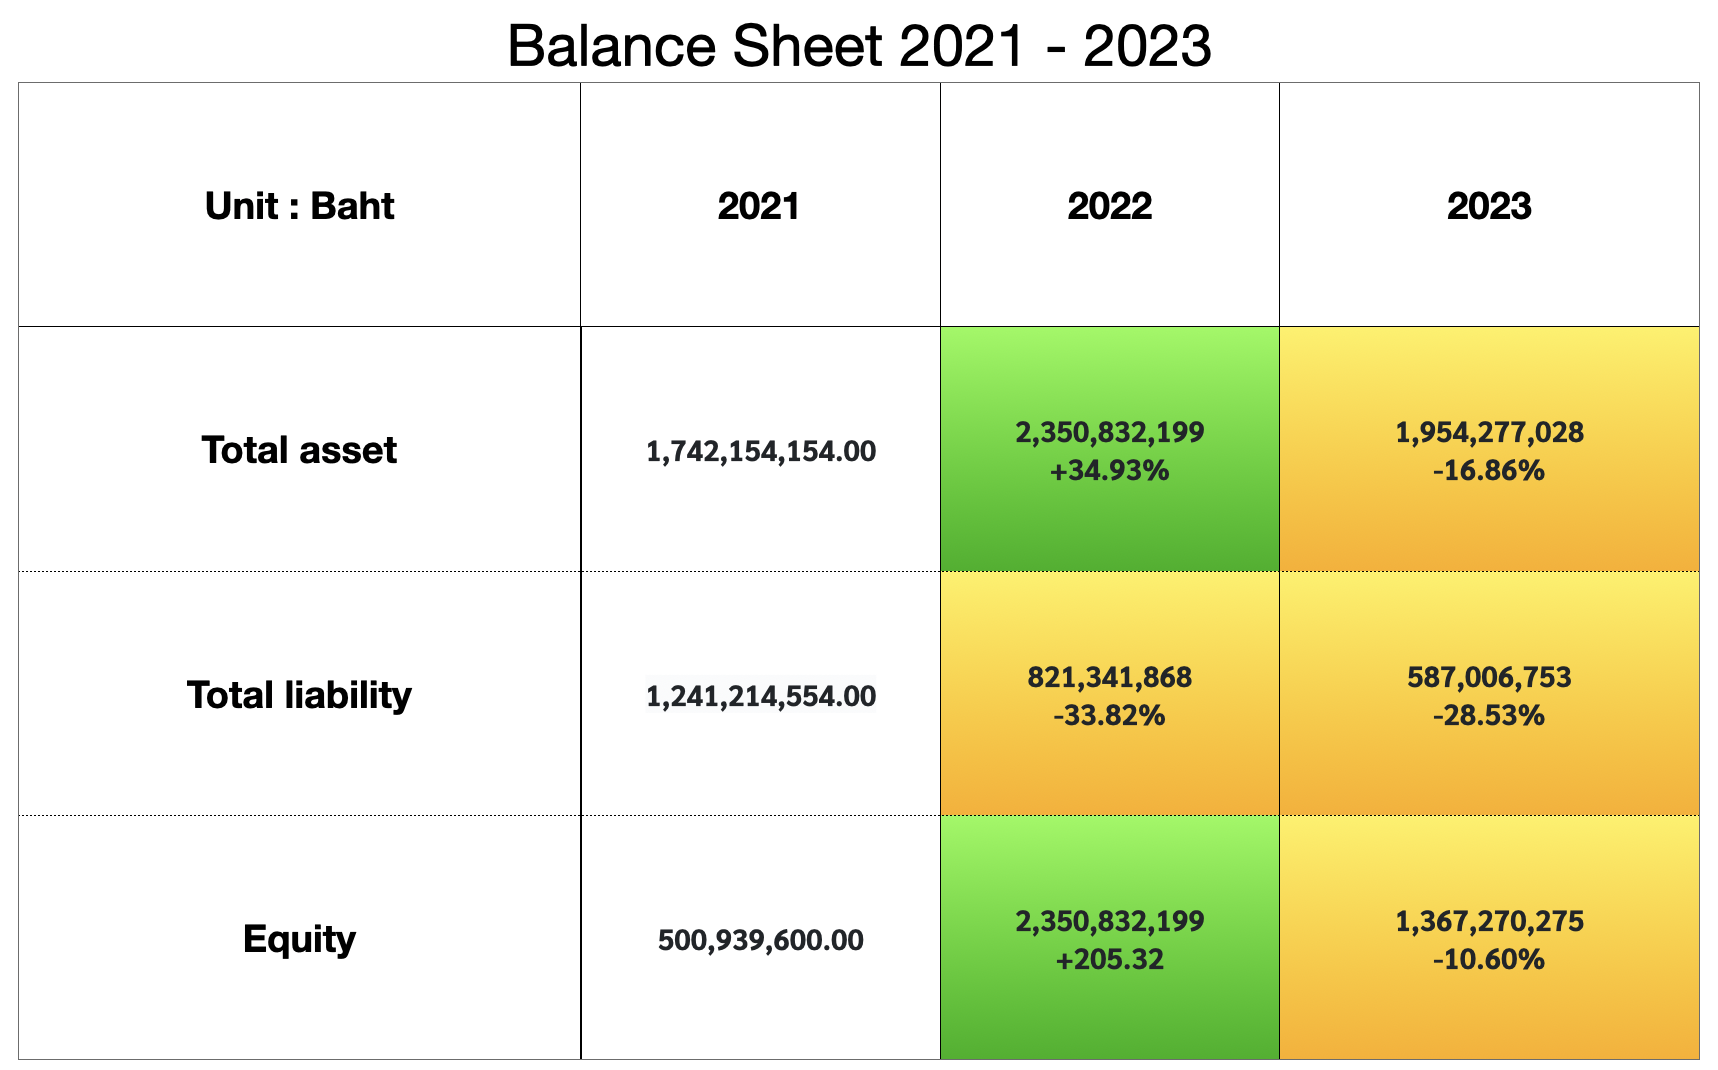
\includegraphics[scale=0.4]{images/balance.png}
    \end{center}
    \caption[งบการเงินย้อนหลังตั้งแต่ก่อตั้งบริษัท]{งบการเงินย้อนหลังตั้งแต่ก่อตั้งบริษัท}
\end{figure}
เนื่องจากบริษัท SCB TechX เป็นบริษัทในเครือของ SCB ดังนั้นจึงจะเห็นว่าทรัพย์สินของบริษัทนั้นมีมูลค่าสูงหลักพันล้านบาท ตั้งแต่เริ่มก่อตั้งบริษัท ทั้งนี้หากมองลึงลงไปในปีแรกก็จะเห็นว่าทรัพย์สินหลักพันล้านนั้นเกิดมาจากการกู้ยืมเป็นส่วนใหญ่ ในส่วนของผู้ถือหุ้นนั้นยังไม่มากในช่วงแรก หากอ้างอิงข้อมูลจากใน \textit{รูปที่ 1.2 }แล้วนั้นจะเห็นได้ว่าในปีที่สองมูลค่าทรัพย์สินรวมเพิ่มสูงขึ้นอย่างก้าวกระโดด ทั้งนี้ด้วยการเติมโตที่อาจจะเร็วเกินไปทำให้ในปีต่อมาค่อยๆปรับลดลง  แต่มูลค่าหนี้สินจะเห็นได้ว่าค่อยๆลดลงเรื่อยๆ แสดงให้เห็นถึงการพัฒนาของบริษัทได้เป็นอย่างดี

\clearpage

\subsection{งบกำไรขาดทุน}
\begin{figure}[ht]
    \begin{center}
        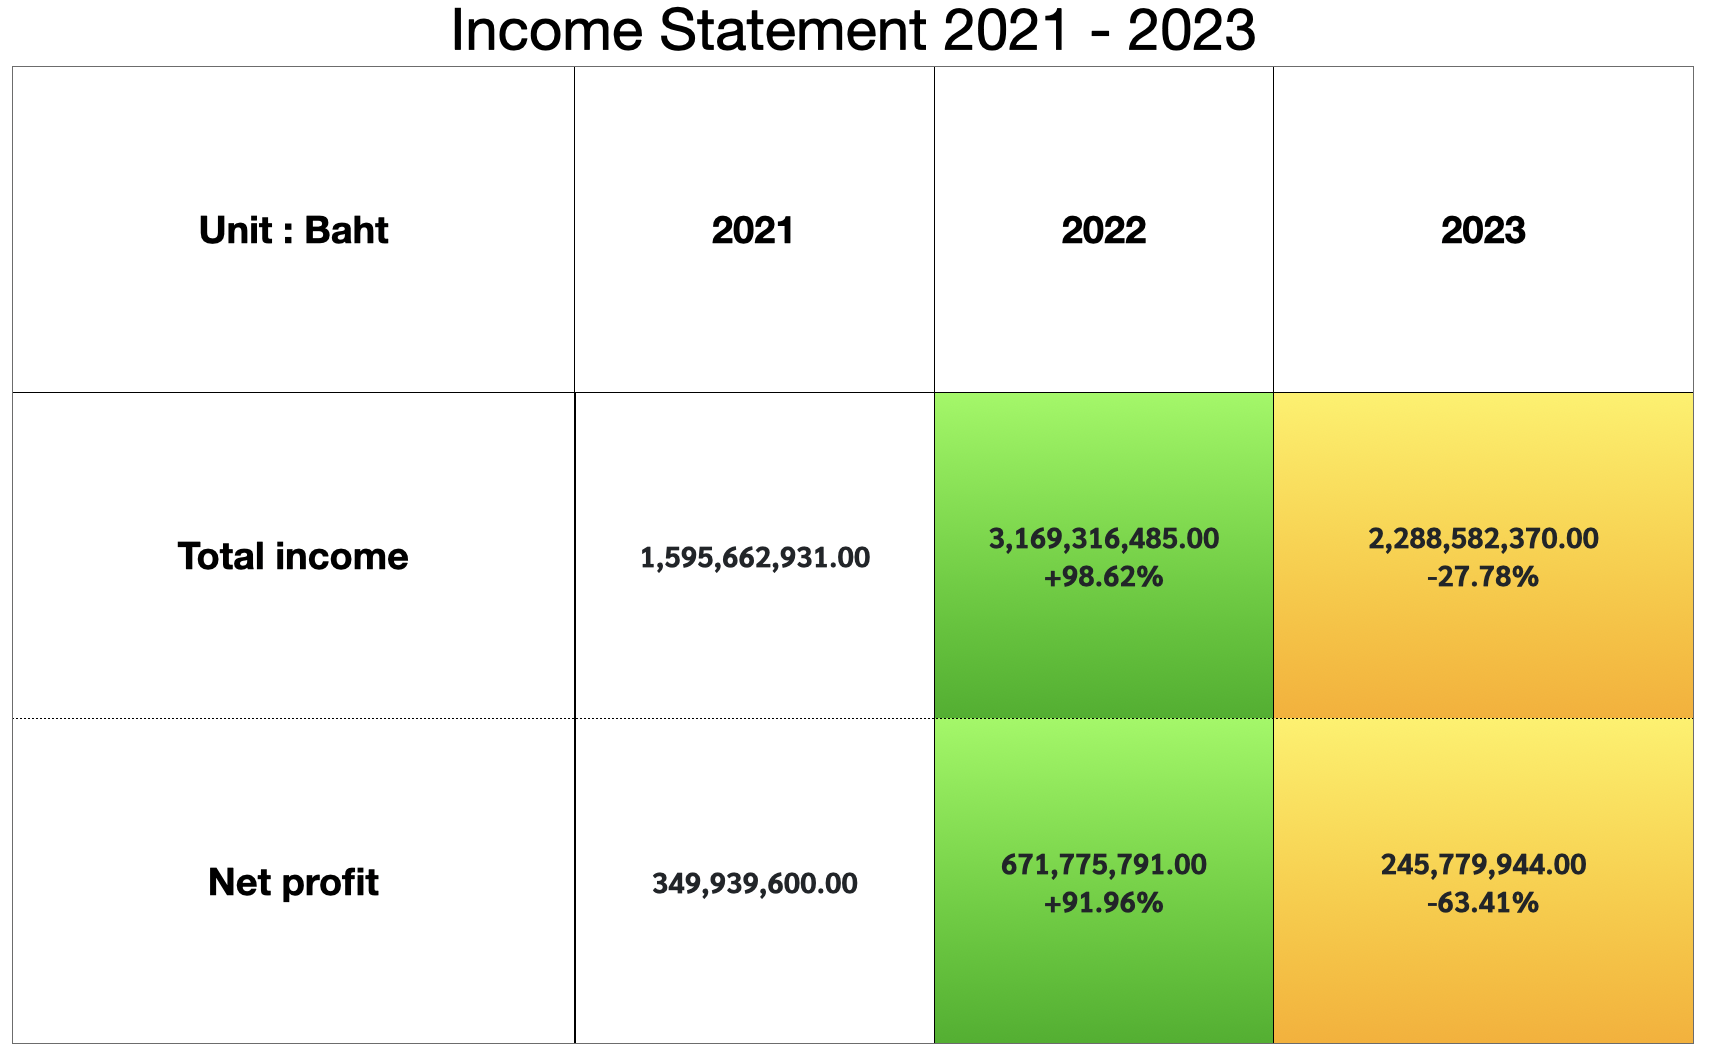
\includegraphics[scale=0.4]{images/profit.png}
    \end{center}
    \caption[งบกำไรขาดทุนย้อนหลังตั้งแต่ก่อตั้งบริษัท]{งบกำไรขาดทุนตั้งแต่ก่อตั้งบริษัท}
\end{figure}
จากข้อมูลใน \textit{รูปที่ 1.3} จะเห็นได้ว่าบริษัท SCB TechX มีกำไรตั้งแต่ปีที่สอง และกำไรเพิ่มขึ้นอย่างมีนัยสำคัญ ถึงแม้ในปี 2023 กำไรลดลงจากปี 2022 ถึง ร้อยละ 63 เป็นเพราะการพัฒนาของบริษัทที่เร็วขึ้น การขยายขนาดของบริษัท ทำให้ต้องเพิ่มการจ้างงานมากขึ้นจึงเป็นเหตุที่ทำให้รายได้ลดลงจากปีก่อนหน้า แต่ถ้าหากเปรียบเทียบกับปีแรกก็ยังถือว่ามีกำไรอยู่ในระดับที่ดีในทุก ๆ ปี


\section{หน้าที่ของหน่วยงานที่ได้มาสหกิจ}
ในตำแหน่ง DevOps Engineer ที่ SCB TechX หน้าที่หลักของผมคือการทำงานเป็นตัวกลางระหว่างทีมพัฒนา (Development Team) และทีมปฏิบัติการ (Operation Team) โดยมุ่งเน้นไปที่การพัฒนาและจัดหาเครื่องมือเพื่อช่วยในการบริหารจัดการระบบ รวมถึงสนับสนุนการทำงานของทีมพัฒนา นอกจากนี้ ยังมีบทบาทสำคัญในการดูแลและปรับปรุงกระบวนการ CI/CD เพื่อให้การส่งมอบระบบไปยังผู้ใช้ (Delivery) เป็นไปอย่างราบรื่นและรวดเร็ว

ในด้านอื่น ๆ ผมยังมีหน้าที่ในการเตรียมความพร้อมของ Pipeline สำหรับการ Deploy และสร้างเครื่องมืออัตโนมัติ (Automation Tools) เพื่อช่วยลดเวลาทำงานของทุกทีมในองค์กร อีกทั้งยังทำหน้าที่ประสานงานเกี่ยวกับเครือข่าย (Network) และความปลอดภัย (Security) เพื่อสนับสนุนทีมอื่น ๆ ภายในบริษัทตามขอบเขตงานที่ได้รับมอบหมาย